\chapter{Task-Based, Parallel and Distributed Dense Linear Algebra Applications \label{chap:exp_dense}}
\graphicspath{{chapters/exp_dense/}}

The task based programming models we will use to make experiments have been selected in the previous chapter.
We will now introduce the experiments we executed on clusters and supercomputers with the dense linear algebra applications we implemented using these task based programming models.
We will also discuss the numerical experiments we performed and the results we obtained.

\section{Task-Based Methods and Algorithms to Solve Dense Linear Systems}


Let $A$ be a block matrix of size $np \times np$ and $p \times p$ blocks so each block is of size $n \times n$ .
Let $b$ and $x$ be block vectors of size $np$ and $p$ blocks so each block is of size $n$.
The goal here is to solve the linear system $Ax=b$.

In the following algorithms, $A_{i,j}^{(k)}$ represents the $k^{th}$ version of the block at the $i^{th}$ row and $j^{th}$ column of the block matrix $A$.
Thus, $b_i^{(k)}$ represents the $k^{th}$ version of the block at the $i^{th}$ row of the block vector $b$.
The algorithm is expressed using assignments on the blocks of $A_{i,j}^{(k+1)}$ and $b_i^{(k+1)}$.
They consist on operations on blocks like matrix matrix product, inversion of a matrix and matrix vector product.
Each assignment will correspond to a task in the implementation of the algorithms so the number of task will correspond to the number of assignments.




\subsection{Block-Based Gaussian Elimination}

\begin{algorithm}[h]
	\DontPrintSemicolon
	\caption{Block-Based Gaussian elimination and back substitution \label{alg:bg_el_data_dep}}
	%\scriptsize
	\For{k \KwFrom 0 \KwTo p-2}{
		(1) $\displaystyle Inv^{(k)} = [A_{k,k}^{(k)}]^{-1}$ \;
		(2) $b_k^{(k+1)} = Inv^{(k)} \cdot b_k^{(k)}$ \;
		\For{j \KwFrom k+1 \KwTo p-1}{
			(3) $\displaystyle A_{k,j}^{(k+1)} = Inv^{(k)} \cdot A_{k,j}^{(k)} $ \;
		}
		\For{i \KwFrom k+1 \KwTo p-1}{
			(4) $b_i^{(k+1)} = b_i^{(k)} - A_{i,k}^{(k)} \cdot b_k^{(k+1)}$ \;
			\For{j \KwFrom k+1 \KwTo p-1}{
				(5) $A_{i,j}^{(k+1)} = A_{i,j}^{(k)} - A_{i,k}^{(k)} \cdot A_{k,j}^{(k+1)}$ \;
			}
		}
	}

	(6) $b_{p-1}^{(p)} = Inv^{(p-1)} \cdot b_{p-1}^{(p-1)}$ \;

	\For{k \KwFrom 1 \KwTo p-1 }{
		\For{i \KwFrom 0 \KwTo p-k-1 }{
			(7) $b_i^{(k+i+1)} = b_i^{(k+i)} - A_{i,p-k}^{(i+1)} \cdot b_{p-k}^{(p)}$ \;
		}
	}
\end{algorithm}

The Gaussian elimination in Algorithm \ref{alg:bg_el_data_dep} solves the system by doing a block triangularization of the block matrix $A$, and by solving the triangular system.
In this algorithm, the number of assignments is $\frac{p^3+3p^2+2p}{3} \sim \frac{p^3}{3}$.
The block-wise Gaussian elimination and back substitution have been implemented using YML/XMP.

For this experiments, the Algorithm \ref{alg:bg_el_data_dep} is expressed as YvetteML graph and the operations on blocks are implemented using XMP.
Each operation is performed on a matrix of a vector which are a subdivision of the global matrices and vectors.
In YvetteML, there are two means to express the parallelism between components : the \textit{par} loop and the \textit{par} statement.
To implement the block-wise Gaussian elimination, we expressed all the call to the components in parallel and we used the event management system of YvetteML to express the dependencies between the tasks.
In the Algorithm \ref{alg:bg_el_data_dep}, we observe that each block i,j at step k of the Gaussian Elimination is updated only once.
Then, it is possible to associated the corresponding tasks to the triplets (i,j,k).
Each task may be launched only when some tasks of the previous steps are completed and when the data are migrated to the allocated computing resource.
Therefore, the dependency graph is equivalent in this case of the precedence between triplets: for example (i,j,k) will always depend of (i,j,l$<$k), for the adequate value of i,j, and k.
If we associate each triplet to a Yvette array of events, each assignment of the block (i,j) at step k in the Algorithm \ref{alg:bg_el_data_dep} have to be preceded by a “wait” expressing the dependence between (i,j,k) and previous triplets.
For the block i of a given step  of the back substitution, we use the same properties.

The XMP components that make the different operations are also written to take advantage of the XMP directives and use the processors allocated by YML to efficiently run the operations on the block matrices.



\subsection{Block-Based Gauss-Jordan Elimination}

\begin{algorithm}[h]
	\DontPrintSemicolon
	\caption{Block-Based Gauss-Jordan elimination to solve a linear system \label{alg:bgj_data_dep} }
	\For{k \KwFrom 0 \KwTo p-1}{
		(1) $\displaystyle Inv^{(k)} = [A_{k,k}^{(k)}]^{-1}$ \;
		(2) $b_k^{(k+1)} = Inv^{(k)} \cdot b_k^{(k)}$ \;
		\For{j \KwFrom k+1 \KwTo p-1}{
			(3) $\displaystyle A_{k,j}^{(k+1)} = Inv^{(k)} \cdot A_{k,j}^{(k)} $ \;
			\For{i \KwFrom 0 \KwTo p-1}{
				\If{k $\neq$ i}{
					(4) $A_{i,j}^{(k+1)} = A_{i,j}^{(k)} - A_{i,k}^{(k)} \cdot A_{k,j}^{(k+1)}$ \;
				}
			}
		}
		\For{i \KwFrom 0 \KwTo p-1}{
			\If{k $\neq$ i}{
				(5) $b_i^{(k+1)} = b_i^{(k+1)} - A_{i,k}^{(k)} \cdot b_k^{(k+1)}$ \;
			}
		}
	}
\end{algorithm}

\subsection{Block-Based LU factorization}

\begin{algorithm}[h]
	\DontPrintSemicolon
	%\SetAlgoVlined
	\caption{LU Factorization\label{alg:lufact_data_dep}}
	\For{k \KwFrom 0 \KwTo p-2}{
		(1) $\displaystyle Inv^{(k)} = [A_{k,k}^{(k)}]^{-1}$ \;
		\For{i \KwFrom k+1 \KwTo p-1}{
			(2) $\displaystyle A_{i,k}^{(k+1)} = A_{i,k}^{(k)} \cdot Inv^{(k)}$ \;
			\For{j \KwFrom k+1 \KwTo p-1}{
				(3) $A_{i,j}^{(k+1)} = A_{i,j}^{(k)} - A_{i,k}^{(k+1)} \cdot A_{k,j}^{(k)}$ \;
			}
		}
	}
\end{algorithm}

\begin{figure}[h]
	\centering
	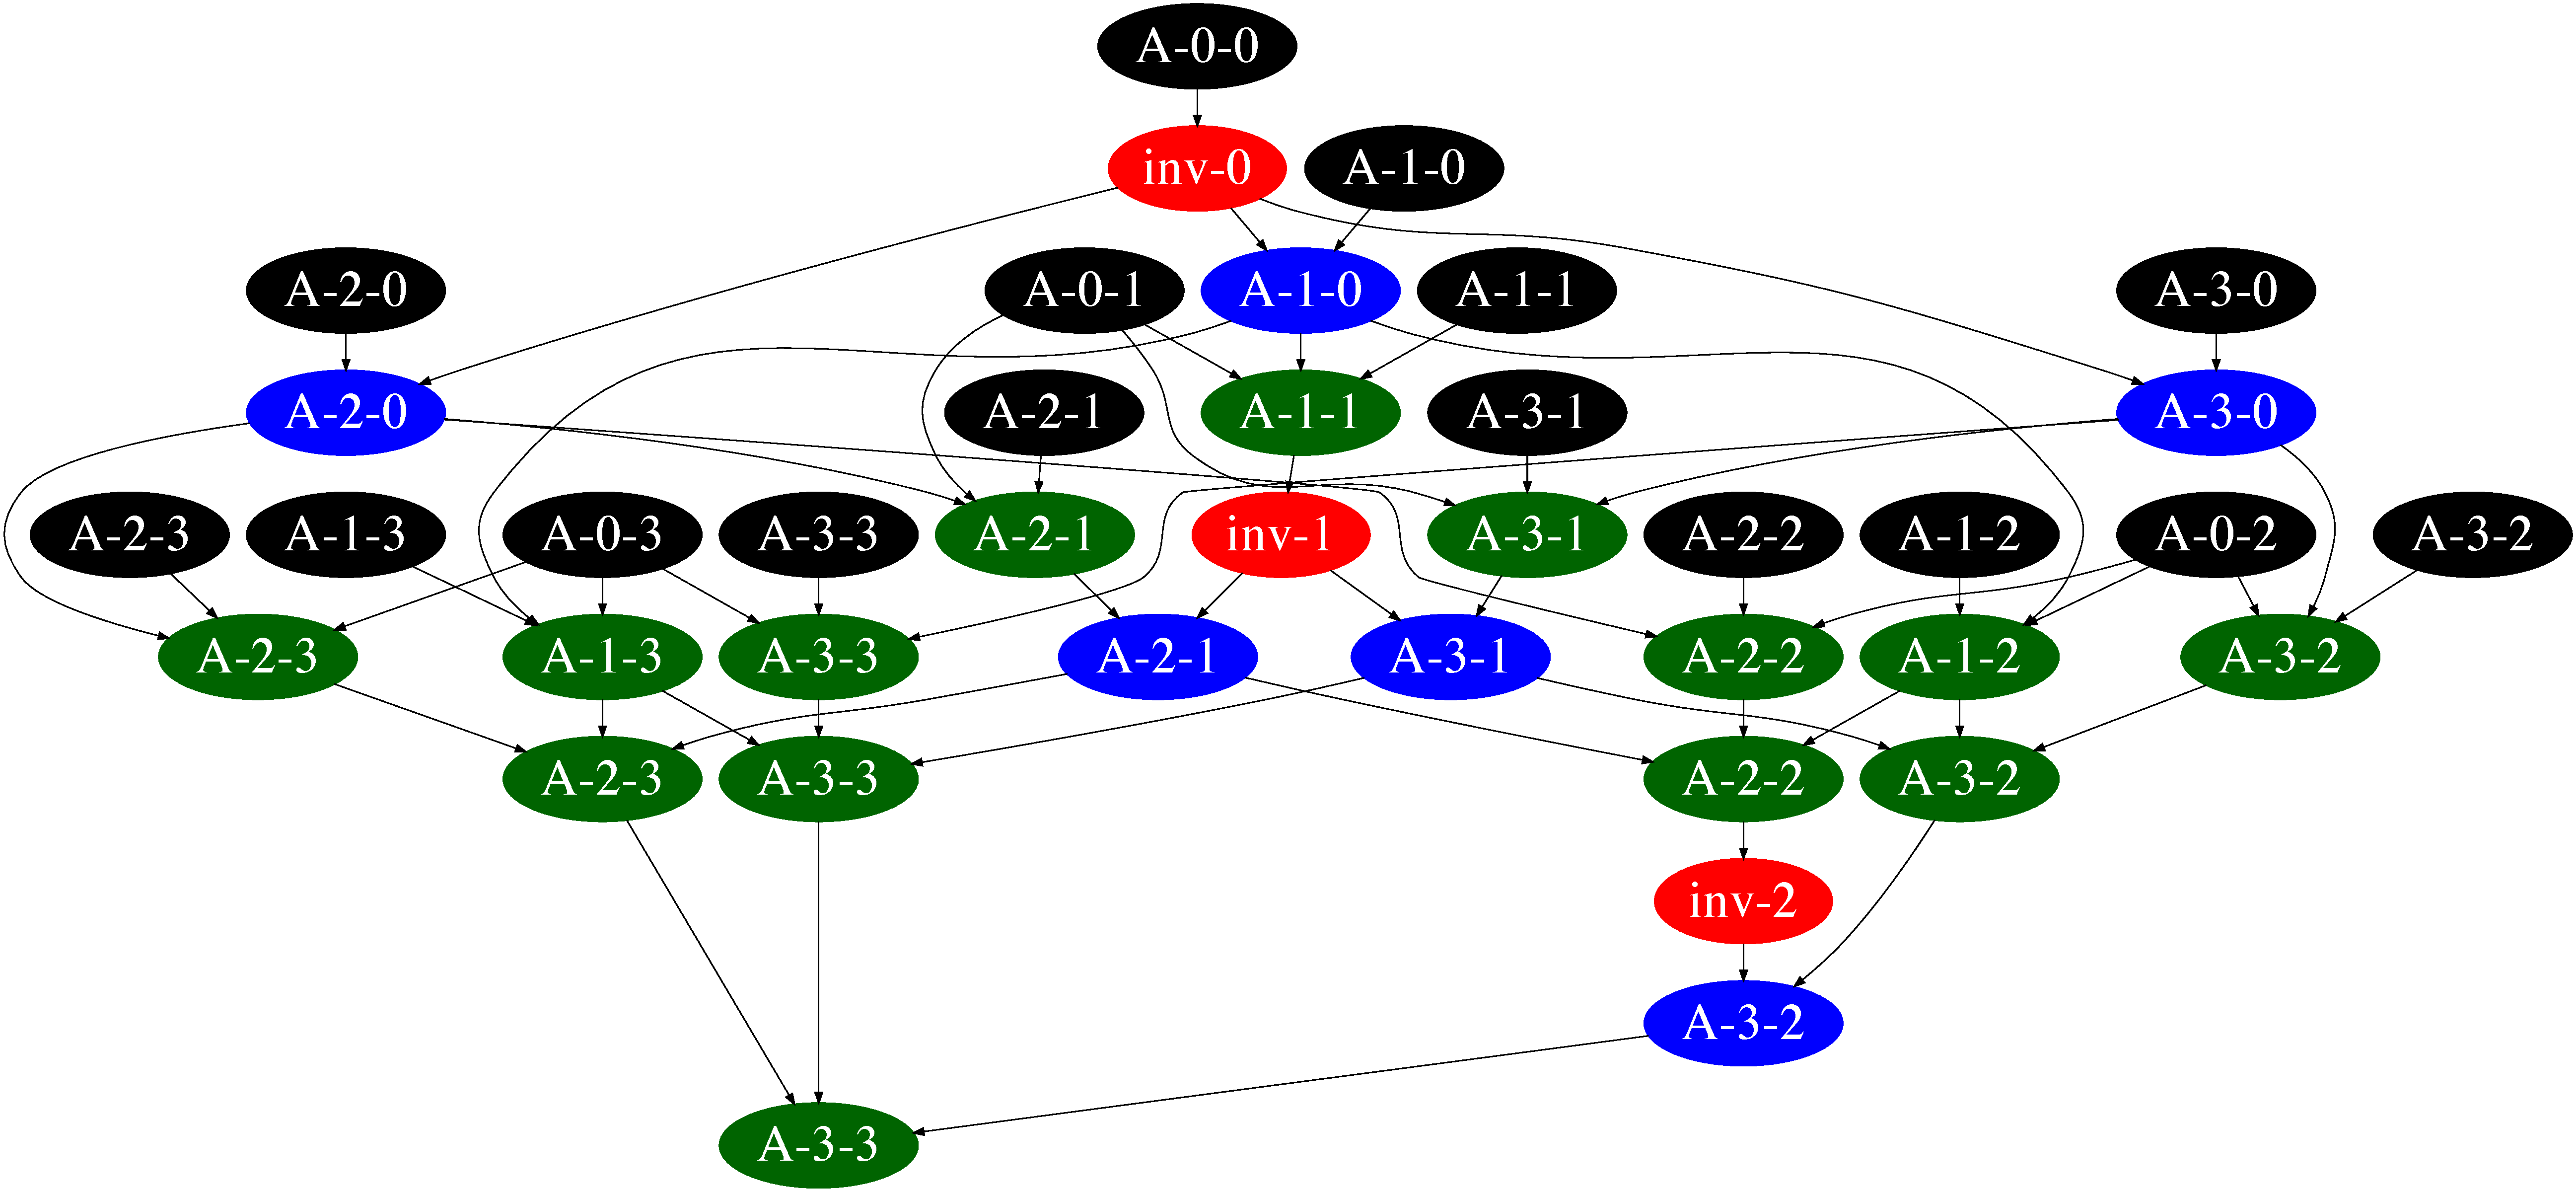
\includegraphics[width=\textwidth]{lu_graph_n4}
	\caption{Block-based LU factorization graph for p = 4\label{fig:graph_lu}}
\end{figure}

\subsection{Block-Based Resolution of Block Triangular Systems}

\begin{algorithm}[h]
	\DontPrintSemicolon
	%\SetAlgoVlined
	\caption{Solution of a linear system with a block-based LU factorization\label{alg:lufact_sls_data_dep}}
	\For{i \KwFrom 0 \KwTo p-2}{
		\For{j \KwFrom i+1 \KwTo p}{
			(5) $b_j^{(i+1)} = b_j^{(i)} - A_{j,i}^{(i+1)} \cdot b_i^{(p)}$ \;
		}
	}
	\;
	\For{k \KwFrom p-1 \KwTo 0 \KwStep -1}{
		(6) solve $b_{k}^{(p)} = A_{k,k}^{(k)} \cdot b_k^{(p-1)}$ \;
		\For{i \KwFrom 1 \KwTo k-1}{
			(7) $b_i^{(p-k+i)} = b_i^{(p-k+i-1)} - A_{i,k}^{(i)} \cdot b_k^{(p)}$ \;
		}
	}
\end{algorithm}


\section{Numerical Experiments on Linear systems}

In the first place, the multi-level programming YML/XMP will be compared to XMP on the K computer where OmniRPC and XMP are installed.
Then, YML/XMP and XMP will be compared to ScaLAPACK and the implementation of the resolution of a dense linear in MPI on Poincare.


\subsection{Experiments on the K computer}

\subsubsection{The supercomputer}
In this section, the tests were performed on the K Computer from Riken AICS in Kobe, Japan.
This supercomputer was manufactured by Fujitsu.
There is 88,128 compute nodes containing an eight-core SPARC64 VIIIfx processor and 16 Go of memory.
The network is based on Tofu interconnect.

\subsubsection{Resolution of a linear system of size 16384 on 1024 cores}
This experiment consists in solving a dense linear system of size 16384 with the block-wise Gaussian elimination with YML/XMP.
The matrix is already generated and each YML task has to load its data from the file system, makes the computations on the data then saves its results to the file system.
The matrix is stored by blocks and each task makes an operation on blocks of the global matrix.
YML expresses the operations on blocks while XMP is used to implement them.
We experiment different numbers of blocks and numbers of cores per task.
Only one process runs on each core.
We used from $1\times 1$ block to $16\times 16$ blocks with tasks from 16 to 512 cores out of the 1024 cores of the K Computer allocated to each run.
The time needed to solve the linear system without the generation of the matrix is evaluated in this study.

\begin{figure}[h]
	\caption{Resolution of linear system using Gaussian elimination + back substitution (size of 16384) on the K computer\label{fig:K_g}}
	\centering
	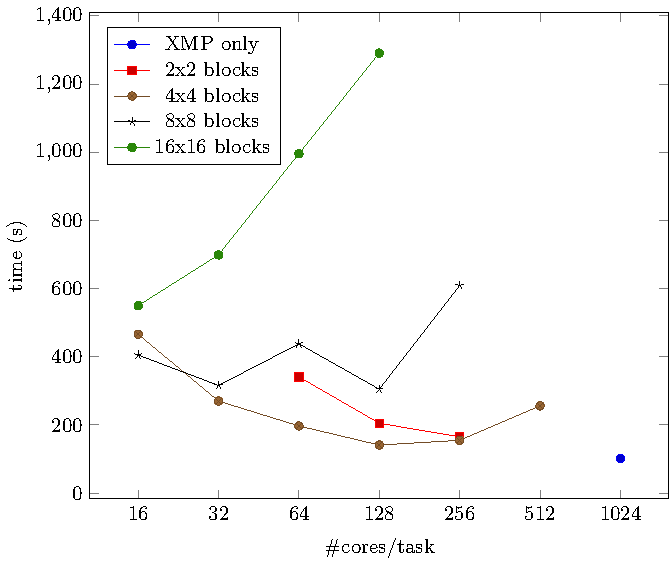
\includegraphics[width=.6\textwidth]{figK-g-16k.pdf}
\end{figure}

\begin{figure}[h]
	\caption{Resolution of linear system using Gauss-Jordan elimination (size of 16384) on the K computer\label{fig:K_gj}}
	\centering
	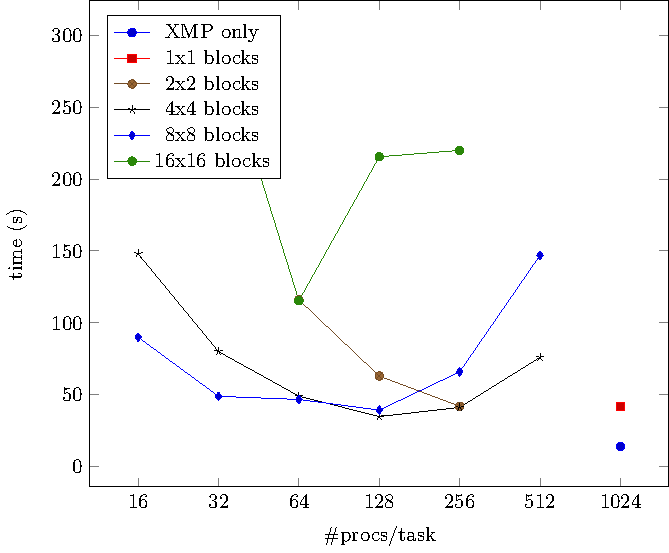
\includegraphics[width=.6\textwidth]{figK-gj-16k.pdf}
\end{figure}

\begin{figure}[h]
	\caption{Resolution of linear system using LU factorization + forward and backward substitution (size of 16384) on the K computer\label{fig:K_lu}}
	\centering
	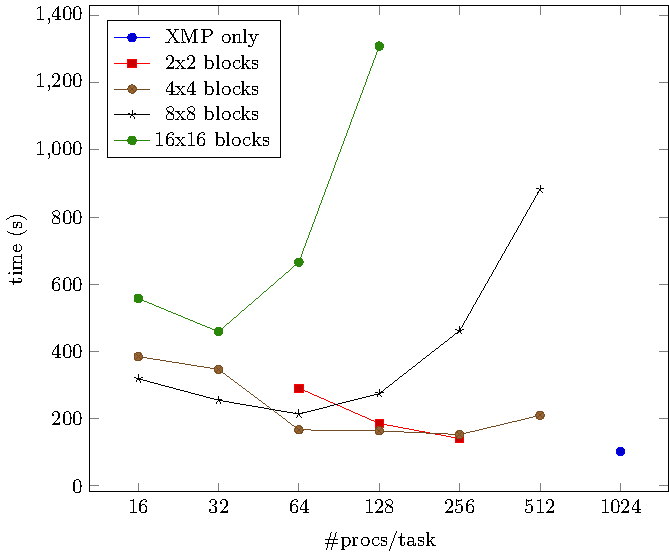
\includegraphics[width=.6\textwidth]{figK-lu-16k.pdf}
\end{figure}

In the Figure \ref{fig:K_g}, we observe the impact of the number of blocks and the number of cores per task on the execution time for the Gaussian elimination.
We also observe the same kind of behavior for the two other applications using different methods to solve the same linear system : the Gauss-Jordan elimination in Figure \ref{fig:K_gj} and the LU factorization in Figure \ref{fig:K_lu}.
We also compare the YML/XMP application to a XMP implementation of the resolution of a linear system through the non-block Gaussian elimination.
We reached the best time in YML/XMP with $4 \times 4$ blocks and 128 cores per task for 141s while the XMP code took 102s.

\textbf{The number of blocks} determines the number of tasks in the application.
For $p \times p$ blocks, there are $\frac{p^3+3p^2+2p}{3}$ tasks in the Gaussian elimination application.
Thus, the application needs to have enough tasks to contain enough parallelism without decreasing to significantly the execution time of each task.
The number of blocks also influences the size of the block since the size of a block is $16384/p \times 16384/p$ values for the matrices and $16384/p$ values for the vectors in the case of a linear system of size 16384.
If the number of blocks is large then the size of the block is small and the tasks on the blocks will be quick.
In the opposite, a small number of blocks implies a large size of blocks so the task will be longer since it will need more operations.
Moreover, if the application has too many tasks, the tasks execution will not compensate the overhead from YML.

\textbf{The number of cores per task} sets the number of YML workers since all the tasks use the same amount of cores and the total number of cores is fixed.
Each worker launches a task at a time so there is the same number of parallel tasks as there is number of workers.
For instance, we use 1024 cores in total and 128 cores per task so there are 8 parallel tasks maximum.
The number of blocks needs to be high enough to use all the workers most of the time or there is unused compute power and the application will take more time.
The number of cores per task also influences the speed of the execution of a task since a large number of cores will have more compute power but will also introduce more communications between cores.
On the opposite, a small number of cores will induce less communications but the task will take more time.

\textbf{A compromise} between the number of blocks and the number of cores per task is mandatory to obtain good performances.
The number of blocks gives enough tasks so there is a great number of those tasks that can be run in parallel and determines the size of the data in the task.
The number of cores per task gives the number of parallel workers and the execution time of each task.
The good compromise gives enough parallel tasks so the workers are busy most of the time and the execution time of the tasks is balanced with the size of the data that need to be treated.
It results in applications that use efficiently the available resources.

\begin{table}[h]
	\caption{Execution time (s) to solve a linear system on the K computer with 1024 cores\label{tab:K_1024p_16384n}}
	\centering
	\begin{tabular}{ccccc}
		                         &      \multicolumn{3}{c}{YML/XMP}      &  XMP   \\
		                         &    blocks    & cores/task & best time &        \\ \hline
		  Gaussian elimination   & $4 \times 4$ &    512     &  141.02   & 102.82 \\
		Gauss-Jordan elimination & $4 \times 4$ &    512     &  138.931  & 229.74 \\
		    LU factorization     & $4 \times 4$ &    512     &  141.221  & 103.07
	\end{tabular}
\end{table}


As shown in Table \ref{tab:K_1024p_16384n}, XMP is faster than YML+XMP in solving the linear system without considering the method used.
However, the Gauss-Jordan elimination elimination performs better in YML+XMP than in XMP whereas the Gaussian elimination and the LU factorization are faster in XMP than their counterpart in YML+XMP.
Moreover, the Gauss-Jordan elimination is more compute and communication intensive compared to the LU factorization and the Gaussian elimination and thus, takes more time than the other two in XMP.
Indeed, the operations of the Gauss-Jordan elimination are a bit different from the Gaussian elimination since the operations above the diagonal in the Gaussian elimination are also performed below the diagonal in the Gauss-Jordan elimination.
Hence, there is no resolution of triangular system and is directly solved.
On the other hand, the Gauss-Jordan elimination in YML+XMP has a similar execution time compared to the Gaussian elimination and the LU factorization in YML+XMP.
We think that the number of cores is too small thus the overhead from YML doesn't compensate for direct communications across all the cores in the Gaussian elimination and the LU factorization although it works well for the Gauss-Jordan elimination.
Then, we tried to solve a bigger system on a higher number of cores.


\subsubsection{Resolution of a linear system of size 32768 and 65536 on 8096 cores}
We also made experiments on larger systems with more cores : 32768 and 65536 on 8096 cores.
The Table \ref{tab:K_8096p} summarize the execution times obtained.

\begin{table}[h]
	\caption{Execution time (s) to solve a linear system on the K computer with 8096 cores\label{tab:K_8096p}}
	\centering
	\begin{tabular}{cccccc}
		                                          & Size  &      \multicolumn{3}{c}{YML/XMP}      &   XMP    \\
		                                          &       &    blocks    & cores/task & best time &          \\ \hline
		  \multirow{2}{*}{Gaussian elimination}   & 32768 & $4 \times 4$ &    512     &   276.8   &  508.5   \\
		                                          & 65536 & $8 \times 8$ &    512     &    690    &   2512   \\ \hline
		\multirow{2}{*}{Gauss-Jordan elimination} & 32768 & $4 \times 4$ &    512     &  285.12   & 615.868  \\
		                                          & 65536 & $8 \times 8$ &    512     &  792.737  & 2970.393 \\ \hline
		    \multirow{2}{*}{LU factorization}     & 32768 & $4 \times 4$ &    512     &  332.35   & 505.412  \\
		                                          & 65536 & $8 \times 8$ &    512     &  881.032  & 2306.163
	\end{tabular}
\end{table}

In this experiment, we increased the size of the system and the number of cores.
In this case, YML/XMP performed better than XMP alone for the two different size for each application.
This is mainly due to the fact that YML doesn't make any global communications like broadcast over all the cores allocated to the application.
Indeed, each task runs on a subset of the resources and the communications between tasks are made through the data server.
Although, the overhead of YML is noticeable (this will be discussed in the next section), YML+XMP runs faster than XMP alone on 8096 cores of the K Computer.
Thus YML+XMP and the task programming languages may be a good solution to develop and execute complex applications on huge numbers of cores on large super-computers.

In this case, where the size of the problem and the number of computational resources has increased, the Gaussian elimination in YML+XMP is noticeably faster than the LU factorization and the Gauss-Jordan elimination in YML+XMP whereas the three of them were equivalent in the previous case.
Moreover, the Gaussian elimination and the LU factorization have almost the same number of tasks but the Gaussian elimination executes faster.
Indeed, the critical path of the Gaussian elimination is shorter than the critical path of the LU factorization due to the fact that, in the LU factorization, there is two triangular systems to solve while there is only one in the Gaussian elimination.
The Gauss-Jordan elimination also performs better than the LU factorization although there is more computation but the critical path is even shorter than the critical path of the Gaussian elimination.
We think that with greater sizes of problem and number of computational resources, the discrepancy between the LU factorization and the Gaussian elimination will increase whereas it will decrease between the Gauss-Jordan elimination and the Gaussian elimination.
The Gauss-Jordan elimination may even execute faster than the Gaussian elimination at some point.


We compared YML/XMP to XMP for several cases on the K computer to evaluate the multi-level distributed/parallel programming associated to the studied programming paradigm on such supercomputer, even if the system of these machines does not yet propose smart scheduling.
As YML and XMP were introduced by authors of this paper, as the OmniRPC middleware used fore these experiments, we have to evaluate such programming on a more general cluster and compare it to more classic end-user programming.
Then, in the next section, we compare YML/XMP and XMP to ScaLAPACK and our MPI implementation of the resolution of a dense linear system on Poincare, an IBM cluster.


\subsection{Experiments on Poincare, a cluster from La Maison de la Simulation\label{sec:exp}}

\subsubsection{The cluster}
The tests were performed on Poincare, the cluster of \textit{La Maison de la Simulation} in France.
It is an IBM cluster mainly composed of iDataPlex dx360 M4 servers, hosted at the CNRS supercomputer centre in Saclay, France.
There is 92 compute nodes with 2 Sandy Bridge E5-2670 processors (8 cores each, so 16 cores per nodes) and 32 Go of memory.
The file system is constituted of two parts : a replicated file system with the homes of the users and a scratch file system with a faster access from the nodes.
The network is based on QLogic QDR InfiniBand.

\subsubsection{The experiments}
We performed the same tests on YML/XMP as on the K Computer.
We also compared those results to ScaLAPACK, to our custom MPI implementations and $1\times 1$ block in YML/XMP.

In the case of $1\times 1$ block, there is only one assignment performed on a dense linear system with a XMP component.
The component which runs the resolution of linear system is developed using XMP so we can evaluate the time that YML need to schedule the data, import it, run the XMP application then export the data.
The data is loaded from the file system.
This is the worst case for YML since it does not use the advantages of YML like scheduling and high grain parallelism.

We also compare the YML/XMP implementation of the Gaussian elimination, the Gauss-Jordan elimination and the Lu factorization to a XMP and a MPI implementations.
Finally, we also compare to a ScaLAPACK implementation of the resolution of a dense linear system through LU factorization.
In each case, we load the data from disk using MPIIO then we solve the linear system and save the result vector on disk using MPIIO.

In the MPI case, we used a cyclic distribution of the columns to keep a good load balancing in the cores.
Moreover, we created a distributed cyclic array type in MPI in order to use it with MPIIO.
This results in a matrix well stored by columns in the file.
The cyclic distribution takes more time since it is easier to store the data without reordering them during the import/export.

\subsubsection{The results}

\begin{figure}[h]
	\caption{Resolution of linear system using Gaussian elimination + backward substitution (size of 16384 on the left and 32768 on the right) on Poincare\label{fig:g1}}
	\centering
	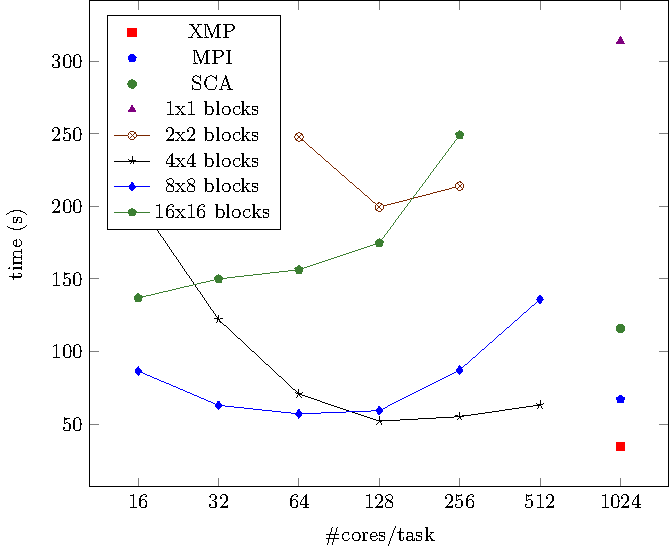
\includegraphics[width=.49\textwidth]{fig-g-16k.pdf}
	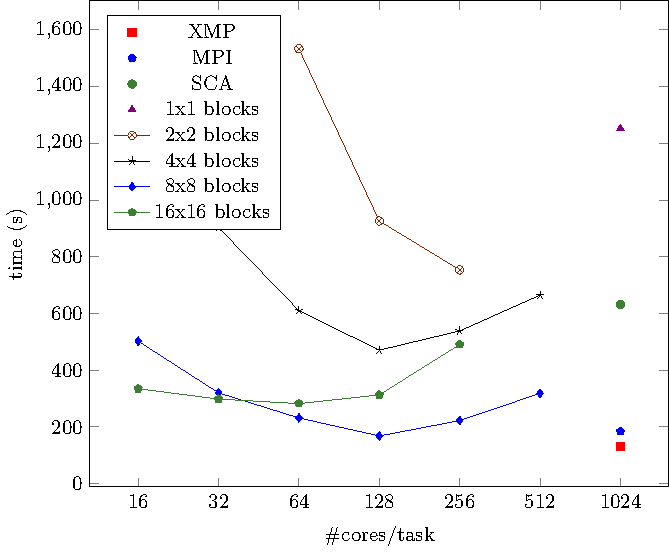
\includegraphics[width=.49\textwidth]{fig-g-32k.pdf}
\end{figure}

The Figure \ref{fig:g1} shows the performances to solve a linear system of size 16384 and 32768 by the block Gaussian elimination and the block resolution of the resulting triangular system using YML/XMP.
The best execution time for YML/XMP is obtained with $4 \times 4$ blocks and 128 cores per tasks for 51.9s for the size of 16768.
The $1 \times 1$ block case with YML/XMP takes more time than the XMP only program (34.5s vs 313s).
We also obtain similar results with the LU factorization (see Figure \ref{fig:lu_poincare}) and the Gauss-Jordan elimination (see Figure \ref{fig:gj}).

The Table \ref{tab:best_time_poincare} gives a summary of the results obtained with the different programming paradigms.
We have the values for two sizes of system 16384 and 32768.
Moreover, for the MPI, XMP and ScaLAPACK cases, we also have the time spent in computation between parenthesis.
The rest of the time is spent in IO to load and save the data as it is done for each component in YML/XMP.

\begin{figure}[H]
	\caption{Resolution of linear system using LU factorization + backward and forward substitution (size of 16384 on the left and 32768 on the right) on Poincare\label{fig:lu_poincare}}
	\centering
	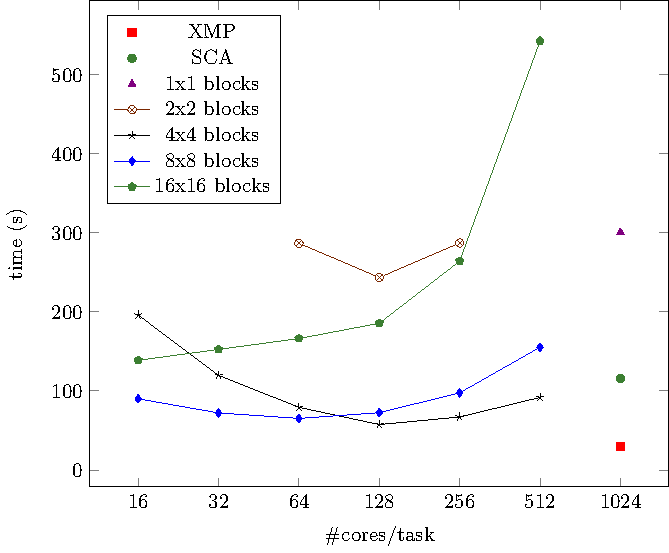
\includegraphics[width=.49\textwidth]{fig-lu-16k.pdf}
	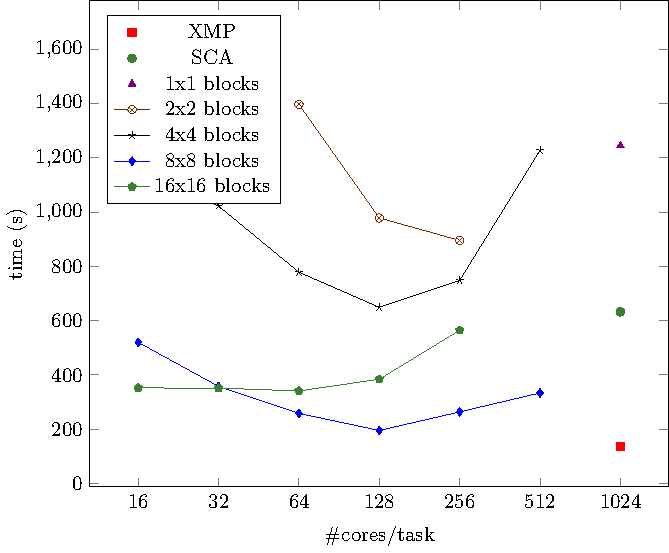
\includegraphics[width=.49\textwidth]{fig-lu-32k.pdf}
\end{figure}

\begin{figure}[h]
	\caption{Resolution of linear system using Gauss-Jordan elimination (size of 16384 on the left and 32768 on the right) on Poincare\label{fig:gj}}
	\centering
	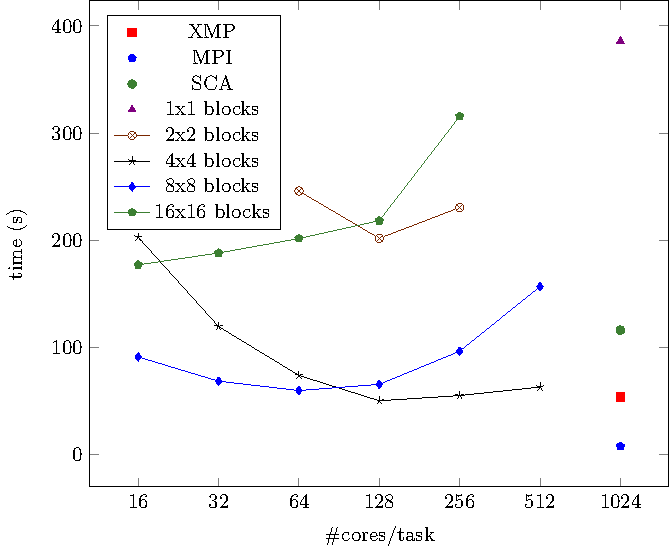
\includegraphics[width=.49\textwidth]{fig-gj-16k.pdf}
	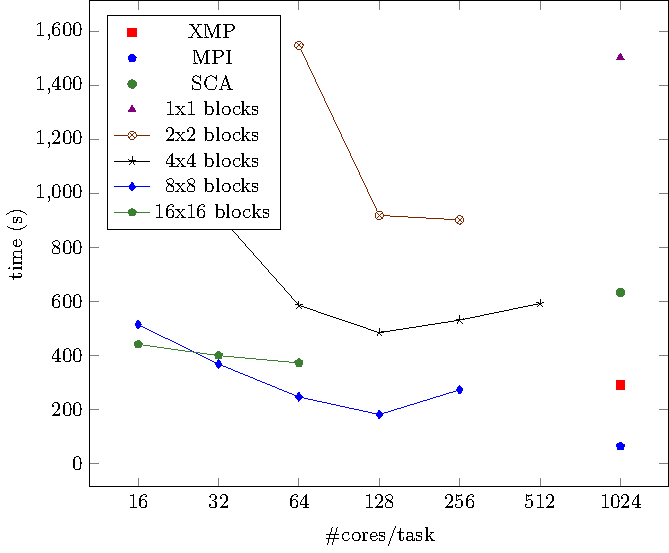
\includegraphics[width=.49\textwidth]{fig-gj-32k.pdf}
\end{figure}


With the Gauss-Jordan method, YML/XMP runs faster than XMP on Poincare for the two sizes of systems and the difference increases with the size of the system.
We observe the same effect of balance between the number of cores per task and the number of blocks as we seen previously.
The parallelism inside the Gauss-Jordan elimination is greater so the task parallel programming paradigm take advantage of this parallelism to execute the application.
Moreover, there is no global communications in YML/XMP but they are widely used in XMP so the increase of operations from the Gaussian elimination to the Gauss-Jordan elimination is more impacting in XMP.
Our MPI implementation is unexpectedly quite fast on a system of size 163824 but ScaLAPACK is more efficient in term of computation for the 32768 system.
Finally, the Gaussian elimination performed almost two times better on XMP than the Gauss-Jordan elimination but the two methods got very close results on YML/XMP.

\begin{table}[h]
	\caption{Execution time (s) to solve a linear system\label{tab:best_time_poincare}}
	\centering
	\begin{tabular}{cccc}
		                                          &           Language           &    16384     &      32768      \\ \hline
		  \multirow{5}{*}{Gaussian elimination}   &     YML/XMP (best case)      &     51.9     &      168.3      \\
		                                          & YML/XMP ($1 \times 1$ block) &     313      &      1252       \\
		                                          &             MPI              & 66.9 (60.6)  &  183.7 (161.9)  \\
		                                          &             XMP              & 34.5 (32.7)  &  131.4 (129.6)  \\
		                                          &          ScaLAPACK           & 115.9 (18.5) &  632.1 (55.6)   \\ \hline
		    \multirow{4}{*}{LU factorization}     &     YML/XMP (best case)      &    57.508    &      194.8      \\
		                                          & YML/XMP ($1 \times 1$ block) &    300.75    &      1244       \\
		                                          &             XMP              & 29.9 (29.4)  & 136.264 (135.6) \\
		                                          &          ScaLAPACK           & 115.9 (18.5) &  632.1 (55.6)   \\ \hline
		\multirow{5}{*}{Gauss-Jordan elimination} &     YML/XMP (best case)      &     49.9     &       180       \\
		                                          & YML/XMP ($1 \times 1$ block) &     385      &      1502       \\
		                                          &             MPI              &  7.4 (4.5)   &    62.1 (59)    \\
		                                          &             XMP              & 53.4 (52.8)  &   289.7 (289)   \\
		                                          &          ScaLAPACK           & 115.9 (18.5) &  632.1 (55.6)
	\end{tabular}
\end{table}

In this case, we globally see the same results although, the Gauss-Jordan elimination has more operations and uses more communications than the Gaussian elimination.
We run faster with YML/XMP than XMP due the parallelism of the method being highly exploited by the parallel task paradigm and not using any global communications.
The efficiency of the YML/XMP depends on the method implemented since the Gaussian elimination and the Gauss-Jordan elimination performed quite close on the two sizes of system while the Gauss-Jordan elimination has a significantly higher number of operations.
The methods with a high parallelism are very suited to the parallel task programming paradigm and perform very well compared to XMP and ScaLAPACK.
The format of the data stored in files by the data server (row-wise) wasn't suited for the distribution of the data used by ScaLAPACK so it didn't performed well as an application.
The use of a better distribution of the data in ScaLAPACK and a data server making IO with the file system in YML/XMP may have shown better performances but YML/XMP and the parallel task programming paradigm show that, even with a high overhead for each task, we can get good performances.


\subsubsection{A comparison between YML/XMP, XMP, MPI and ScaLAPACK}

We can see a huge overhead in YML/XMP for $1 \times 1$ blocks compared to XMP alone in the Table \ref{tab:best_time_poincare}.
This is the case for the two sizes of system and the three applications.
Thus, we can expect a pretty huge overhead from YML for each component.
But, the most favorable case in YML/XMP solve the linear system in 51.9s whereas XMP took 34.5, MPI took 66.9s and ScaLAPACK took 115.9s.
Although, from the 66.9s only 60.6s is spent on computing.
The rest is spent in MPIIO to load and save the data.
In the MPI case, we used a distributed cyclic array so the data in memory and the data on disk are not mapped the same way.
This is why the IO take a bit more time in MPI than XMP since, the data are stored as they are in memory without reordering them.

Moreover, we didn't optimize our MPI implementation to the maximum.
There is a margin of amelioration to get faster results with our MPI implementation.
This implementation is close to the algorithm and use some properties of MPI while trying to reduce the communications between the cores.
In this case, we observe that YML/XMP is slightly faster than our simple MPI implementation and the XMP is relatively close to YML/XMP (It takes 1.58 times more time in the case 16384 and 1.3 in the case 32768).
We can expect that with larger size of systems, YML/XMP will be closer to XMP.

Finally, ScaLAPACK provides the best results if we only consider the computation time as shown in the Table \ref{tab:best_time_poincare}.
Indeed, most of the time is spent in the import of the matrix.
This is due to the distribution of the data in memory.
In this application, ScaLAPACK uses a cyclic distribution of the matrix in a two dimensional grid of cores while the matrix is stored as huge vector representing a row-wise matrix.
Then the values that have to be put in a core are scattered trough the file without any value close to another one.
Thus the import of the matrix is very costly.
ScaLAPACK is the fastest in the of computation time but the import of the matrix from the file system is very costly.
The distribution of the data in this application using ScaLAPACK is not suited for IO.

With a good compromise between the number of blocks and the number of cores per task, we got results relatively close to XMP and MPI.
Moreover, we can expect to get closer results with greater sizes of systems and even get better results at some point.
YML allows more local communications than XMP and MPI.
In YML, the communications are only made on a subset of cores while, in XMP, communications are made across all the cores.
Furthermore, YML has a scheduler that manage the tasks and the data migrations between the tasks in order to optimize them.
They can optimized further with YML asynchronous communications between tasks.
Finally, MPI applications are very well adapted to the current systems so the performances of these applications are great if the application is well implemented.

\subsection{Prediction of the optimal parameters}
The prediction of the optimal values for the number of blocks (size of the block) and the number of processes per task (number of parallel tasks) is not a deterministic problem since it depends on the machine and the available resources.
On a given machine, the job manager will allow the unused resources which differ each time a job is submitted.
Thus, the communications time between two cores will depend on their distance.
The execution time of a task also depends on the loading of the machine since each user can use the network.
Moreover, the computation time has to be higher than the scheduling time so it is worth scheduling the tasks.
The execution time of the application will also depend on the scheduling strategies since it will change the order of execution of the tasks.

The parameters are highly related.
Indeed, the size of a block depends on the number of blocks which influences the total number of tasks.
Furthermore, the size of the block will define the number operation in the task while the number of communications will depend on the number of processes and the size of the block.

Hence, the prediction of the optimal values is difficult but, for a given machine, the machine learning may be able to give an estimation of the value of the parameters.

\section{Numerical Experiments on the LU factorization}
\subsection{Experiments details}
We performed performance tests on up to 64 nodes of Poincare with the LU factorization implemented via MPI, ScaLAPACK, XMP, YML+XMP, HPX, PaRSEC and Regent.
We used several sizes of matrices : $16384 \times 16384$, $32768 \times 32768$ and $49512 \times 49512$.
$16384 \times 16384$ is the largest size we can use to perform the tests on one node since YML+XMP cannot perform the LU factorization with greater sizes of matrices on one node.

In HPX, PaRSEC and Regent, the performances depends on the number of blocks in each dimension (thus, the size of the blocks).
We used several values for the number of blocks.
Table \ref{tab:blocks}, Table \ref{tab:blocks_32k} and Table \ref{tab:blocks_49k} show the block parameters which obtained the fastest execution time for each size of matrix.
The execution times shown here are the case in which we obtained the fastest time for each number of nodes.
We performed those test several times and computed the execution times mean of the same case.
We will compare the results of the task-based programming languages to those obtained with ScaLAPACK.
We will also compare them to our MPI and XMP implementations.
Tests were run on several number of nodes in order to extract strong scaling information which will be discussed in Section \ref{sec:strong_scaling}.
We used  1, 2, 4, 8, 16, 32 and 64 nodes to factorize the $16384 \times 16384$ values matrix.
Then, we used 4, 8, 16, 32 and 64 nodes for the $32768 \times 32768$ values matrix.
And finally, we used 8, 16, 32 and 64 nodes for the $49512 \times 49512$ values matrix.

\begin{table}[h]
	\centering
	\caption{Number of blocks for the fastest case on a $16384 \times 16384$ matrix with number of processes per tasks between parenthesis\label{tab:blocks}}
	\newcolumntype{C}{>{\centering\arraybackslash}X}
\newcolumntype{M}[1]{>{\centering\arraybackslash}m{#1}}
\renewcommand{\arraystretch}{1.2}
\begin{tabularx}{\linewidth}{M{2cm}CCCCCCC}
\\ \hline
& 1 & 2 & 4 & 8 & 16 & 32 & 64 \\ \hline
HPX & $90^2$(1) & $45^2$(1) & $80^2$(1) & $45^2$(1) & $45^2$(1) & $55^2$(1) & $55^2$(1) \\
PaRSEC & $150^2$(1) & $200^2$(1) & $70^2$(1) & $120^2$(1) & $210^2$(1) & $240^2$(1) & $250^2$(1) \\
Regent & $50^2$(1) & $50^2$(1) & $50^2$(1) & $35^2$(1) & $40^2$(1) & $35^2$(1) & $30^2$(1) \\
YML+XMP & $4^2$(8) & $8^2$(8) & $8^2$(16) & $8^2$(32) & $4^2$(128) & $4^2$(128) & $4^2$(128) \\
\hline
\end{tabularx}

\end{table}

\begin{table}[h]
	\centering
	\caption{Number of blocks for the fastest case on a $32768 \times 32768$ matrix with number of processes per tasks between parenthesis\label{tab:blocks_32k}}
	\newcolumntype{C}{>{\centering\arraybackslash}X}
\newcolumntype{M}[1]{>{\centering\arraybackslash}m{#1}}
\renewcommand{\arraystretch}{1.2}
\begin{tabularx}{\linewidth}{M{2cm}CCCCC}
\\ \hline
& 4 & 8 & 16 & 32 & 64 \\ \hline
HPX & $90^2$(1) & $90^2$(1) & $90^2$(1) & $75^2$(1) & $81^2$(1) \\
PaRSEC & $70^2$(1) & $120^2$(1) & $270^2$(1) & $380^2$(1) & $420^2$(1) \\
Regent & $70^2$(1) & $70^2$(1) & $60^2$(1) & $50^2$(1) & $50^2$(1) \\
YML+XMP & $1^2$(64) & $4^2$(64) & $8^2$(32) & $8^2$(128) & $8^2$(128) \\
\hline
\end{tabularx}

\end{table}

\begin{table}[h]
	\centering
	\caption{Number of blocks for the fastest case on a $49512 \times 49512$ matrix with number of processes per tasks between parenthesis\label{tab:blocks_49k}}
	\newcolumntype{C}{>{\centering\arraybackslash}X}
\newcolumntype{M}[1]{>{\centering\arraybackslash}m{#1}}
\renewcommand{\arraystretch}{1.2}
\begin{tabularx}{\linewidth}{M{2cm}CCCC}
\\ \hline
& 8 & 16 & 32 & 64 \\ \hline
HPX & $148^2$(1) & $148^2$(1) & $148^2$(1) & $145^2$(1) \\
PaRSEC & $250^2$(1) & $250^2$(1) & $400^2$(1) & $420^2$(1) \\
Regent & $70^2$(1) & $70^2$(1) & $70^2$(1) & $70^2$(1) \\
YML+XMP & $1^2$(128) & $2^2$(128) & $4^2$(128) & $8^2$(128) \\
\hline
\end{tabularx}

\end{table}

Our MPI application is MPI-only so we used MPI support for shared memory and used one MPI rank per core i.e. 16 processes per core.

ScaLAPACK has a MPI only distributed implementation so it is run with one MPI rank process per core.

Our XMP implementation only uses pure XMP directives which are converted to MPI calls.
It is launched as a MPI only application with one MPI rank process per core.

Regent is a compiler that translates a Lua based code into Legion.
Regent applications are launched by passing the MPI command to Regent launcher which will compile and run the application.
It creates a Legion worker on each node.
Each one of them spawns a process to manage the local tasks, a process to manage data and a process to execute the tasks by default.
Then, the user has to specify the number of processes on which the tasks will be executed.
We used 14 processes on each node to execute the tasks.

To launch our HPX application, we used \textit{mpirun} to execute one instance of HPX runtime on each node.
Then, HPX is able to infer the node configuration.
It spawns a worker process on each core of the node and tasks are run as light-weight threads on those processes.
HPX is able to detect that there is two sockets on the node and manages them internally.

PaRSEC applications were launched with one MPI rank per core.

YML scheduler is launched with MPI on one core (the first one in the machine file) which launch XMP tasks with \textit{MPI\_Comm\_spawn} routine on the leftover cores available.

\subsection{Performances}
\begin{figure}[h]
	\centering
	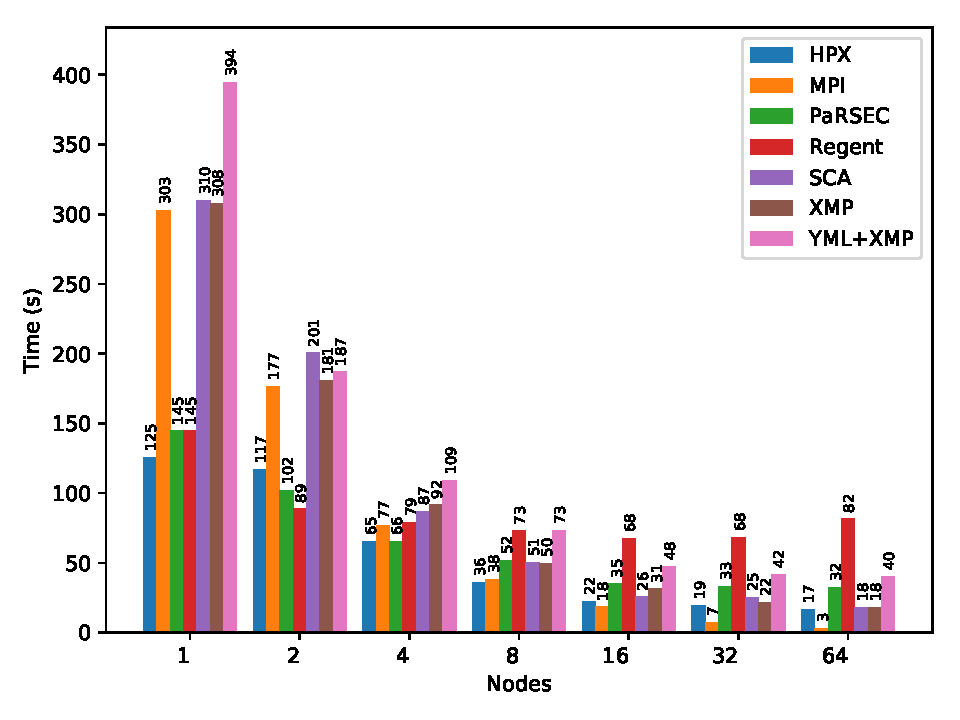
\includegraphics[width=.6\linewidth]{fig_strong_scaling_bar_task}
	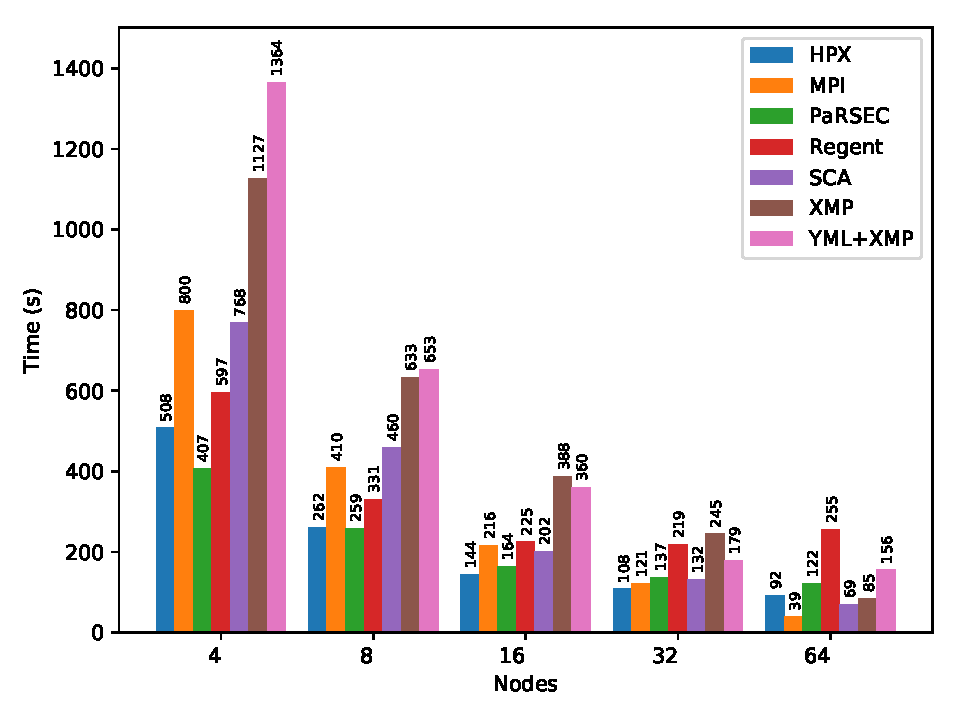
\includegraphics[width=.6\linewidth]{fig_strong_scaling_bar_task_32k}
	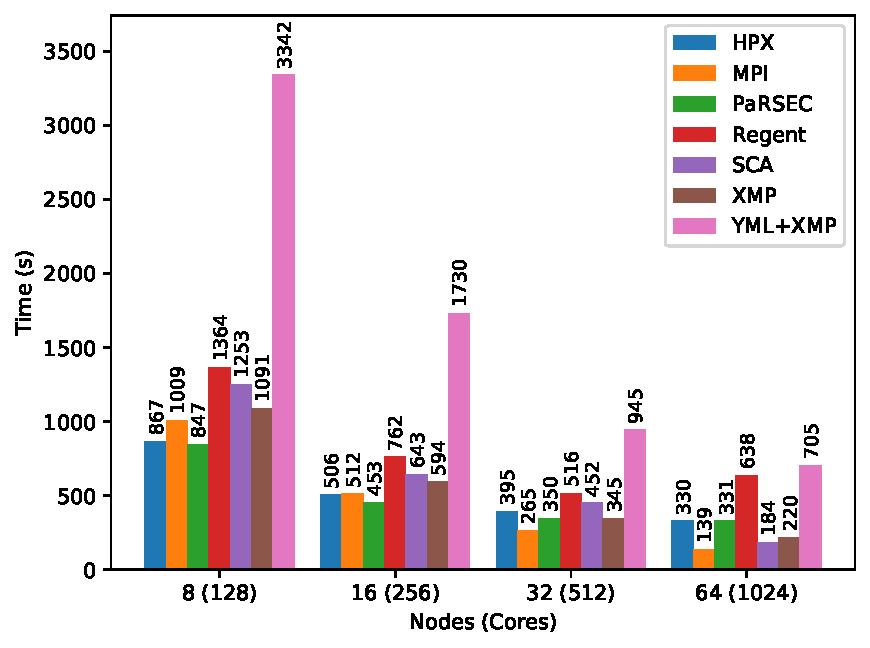
\includegraphics[width=.6\linewidth]{fig_strong_scaling_bar_task_49k}
	\caption{Execution times obtained with the block-based LU factorization implemented with several task-based programming models on a $16384 \times 16384$ matrix (top), a $32768 \times 32768$ matrix (middle) and a $49512 \times 49512$ matrix (bottom)\label{fig:perf}}
\end{figure}


Fig. \ref{fig:perf} shows the performances obtained for the LU factorization with HPX, MPI, PaRSEC, Regent, ScaLAPACK, XMP and YML+XMP on three sizes of matrices $16384 \times 16384$ (top), $32768 \times 32768$ (middle) and $49512 \times 49512$ (bottom).

On a $16384 \times 16384$ matrix, MPI is close to XMP on a small amount of nodes.
When the number of node increases, MPI becomes significantly faster than XMP.
Indeed, Fig. \ref{fig:perf} middle and bottom charts show that MPI is significantly faster than XMP for each number of node.
MPI and XMP applications share the same algorithm and a similar implementation but expressed with two different models.
This may be due to an overhead from the PGAS description and access of the data in XMP compared to MPI.

Regent, HPX and PaRSEC are relatively close to one another on a small number of cores.
However, we can outline tendencies.
PaRSEC is faster than HPX on the lower number of node then HPX becomes faster when the number of node increases.
It also seems that when the size of the matrix increases, HPX and PaRSEC performances are becoming closer and that HPX becomes faster than PaRSEC on the larger number of nodes.
Indeed, HPX becomes faster than PaRSEC after 4 nodes for a  matrix of size $16384 \times 16384$, after 16 nodes for a matrix of size $32768 \times 32768$ and after 64 nodes $49512 \times 49512$.
For the later value, the difference between the two is very small (330s vs 331) so we expect HPX to become significantly faster for this size of matrix with a greater number of nodes.

Regent is a little bit behind HPX and PaRSEC on each number of nodes and size of matrices except for 2 and 4 nodes on a $16384 \times 16384$ matrix where Regent is very efficient.
We can also notice that Regent is taking more time on 64 nodes than on 32.
This may be related to the fact that Regent does not seem to be able to manage a large number of tasks on a large number of nodes since the number of sub-matrices is decreasing when the number of cores is increasing as Table \ref{tab:blocks}, Table \ref{tab:blocks_32k} and Table \ref{tab:blocks_49k} are showing.
However, other task based languages obtain better results when the number of sub-matrices they process increase with the number of cores.
It creates more task and parallelism so that the runtime can use the resources most efficiently.

The YML+XMP applications are the slowest compared to the the applications implemented with the other models.
However, YML+XMP is the only model where tasks are also parallel and distributed.
Moreover, it also uses the file system to perform the communications between the tasks so the communications between tasks are not efficient.

Our last application uses the ScaLAPACK library to compute the LU factorization.
It performs very well on large number of nodes but HPX, PaRSEC and Regent are faster on lower number of cores for each size of matrix.
%TODO confirm
They are not using the same block based algorithm but ScaLAPACK is using a tiled algorithm that makes computations on rows and columns of the matrix \cite{ChDPW1992}.
Therefore, it is an interesting comparison to our block-based algorithms where the operations on the blocks are implemented with tasks.
For a $16384 \times 16384$ matrix ScaLAPACK and HPX are close on 64 nodes but ScaLAPACK is faster for greater size of matrices.
This may be due to the cyclic distribution of data in ScaLAPACK which induces a different communication pattern very efficient on this kind of machine and algorithm.

\subsection{Strong scaling}
\label{sec:strong_scaling}
\begin{figure}[h]
	\centering
	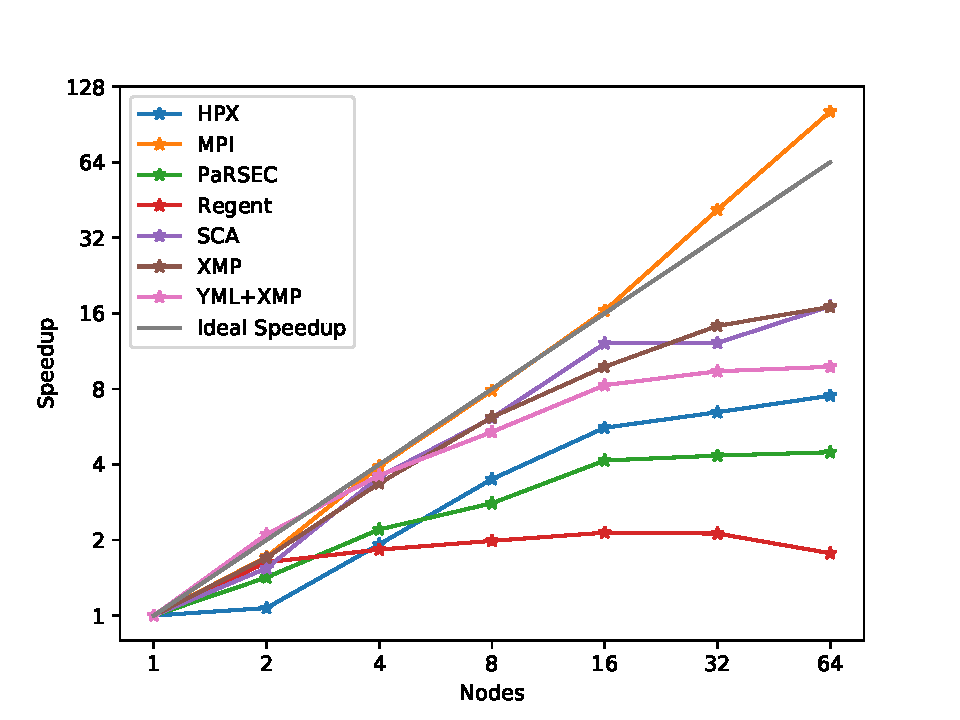
\includegraphics[width=.6\linewidth]{fig_strong_scaling_speedup_task}
	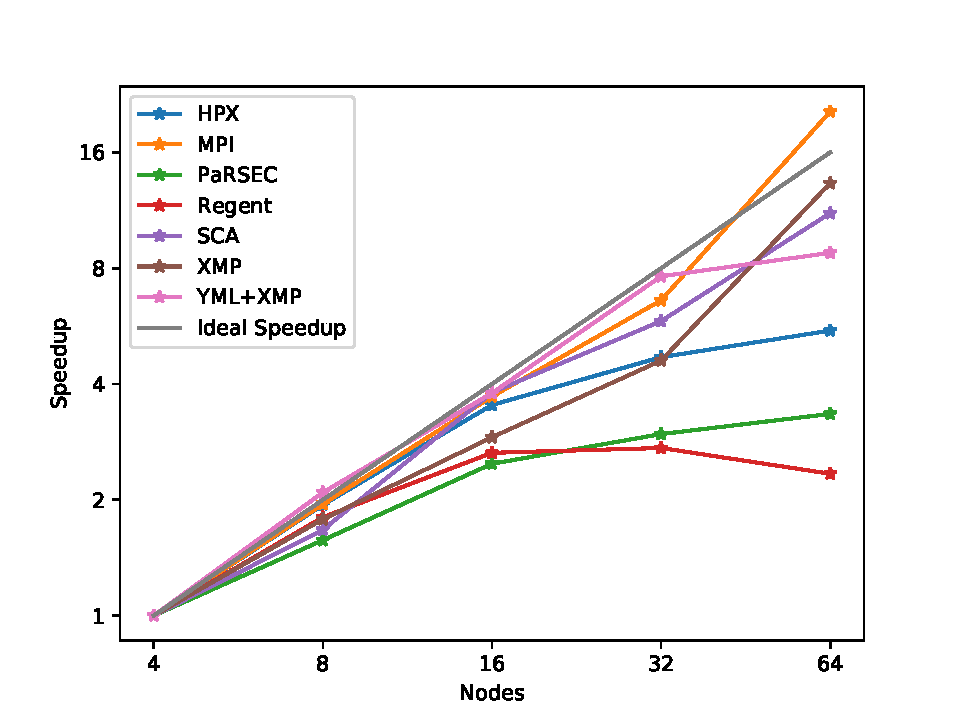
\includegraphics[width=.6\linewidth]{fig_strong_scaling_speedup_task_32k}
	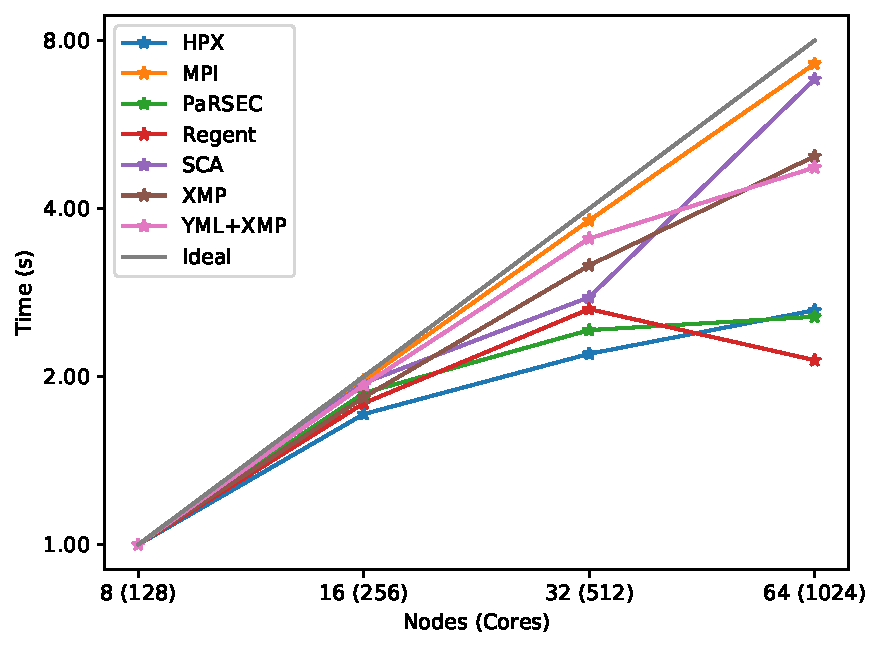
\includegraphics[width=.6\linewidth]{fig_strong_scaling_speedup_task_49k}
	\caption{Speed-ups obtained with the block-based LU factorization implemented with several task-based programming models on a $16384 \times 16384$ matrix (top), a $32768 \times 32768$ matrix (middle) and a $49512 \times 49512$ matrix (bottom) - $log_2$ scale for the y-axis\label{fig:strong_scaling}}
\end{figure}

Fig. \ref{fig:strong_scaling} shows the speed-up extracted from the performances values from Fig. \ref{fig:perf} for HPX, MPI, PaRSEC, Regent, ScaLAPACK, XMP and YML+XMP on three sizes of matrices $16384 \times 16384$ (top), $32768 \times 32768$ (middle) and $49512 \times 49512$ (bottom).
It corresponds to the ratio $t_S/t_N$ where $t_N$ is the execution time for N nodes and $t_F$ is the execution time of the first number of nodes considered in the test.
In the top chart of Fig. \ref{fig:strong_scaling}, $t_F$ is $t_1$ since the experiments start with 1 node.
In the middle (bottom) chart, $t_F$ corresponds to 4 (8).
It translates how efficiently we are managing the addition of more resources to solve the same problem.

Our MPI regular LU factorization is scaling very well as we can see on the charts.
These results are expected since the current systems are well optimized to work with MPI applications.
It even exceeds the ideal speed-up with matrices of size $16384 \times 16384$ (Fig. \ref{fig:strong_scaling} top chart) and $32768 \times 32768$ (Fig. \ref{fig:strong_scaling} middle chart).
We think that it may be due to processes not having enough computations to do on 32 and 64 nodes matrices of size $16384 \times 16384$.
Indeed, when increasing the size of the matrix to $32768 \times 32768$, the strong scalability for our MPI application seems more reasonable.
The same situation occurs for 64 nodes when increasing the size of the matrix from $32768 \times 32768$ to $49512 \times 49512$.

Our task based applications obtain better scalability with the increase of the data size and the number of tasks processed by the applications.
Table \ref{tab:blocks}, Table \ref{tab:blocks_32k} and Table \ref{tab:blocks_49k} show that the number of tasks for a given number of nodes increases with the size of the matrix for each task based programming model.
It produces more parallelism and opportunities to optimize the scheduling of the tasks and improve the use of the computing resources.

Regent strong scalability decreases from 32 to 64 nodes for each size of matrix.
We expect its strong scalability to decrease even more with the increase of the number of cores.

Our HPX application is scaling better than our PaRSEC application with matrices of size $16384 \times 16384$ and $32768 \times 32768$.
It corresponds to the results we obtained in the previous section.
We can also see that PaRSEC and HPX are very close with matrices of size $49512 \times 49512$ and that HPX is exceeding PaRSEC after 32 nodes.
It seems that HPX may have a better scalability than PaRSEC on more than 64 nodes with matrices of size $49512 \times 49512$ if more nodes were available.

Finally, our YML+XMP application has the best strong scalability compared to the other task-based programming models.
As YML+XMP rely on the file system to pass data from one task to another, the performances depends on the efficiency of the file system and its capacity to manage IOs.
Therefore, we think that this programming model will be well adapted to larger machines with a distributed system and integrated schedulers.

\subsection{Results summary}
To conclude, MPI has the best results and scalability on 64 nodes but the application does not use partial pivoting so it is not comparable to ScaLAPACK.
It is also faster than XMP since MPI routines are highly optimized.
Even though, XMP translates its directives into MPI code, the PGAS model used in XMP is not as efficient as using directly MPI.

ScaLAPACK is faster than the applications implemented with the task based programming models but it uses very efficient kernel routines to perform operations internally whereas we are using unoptimized routines.

In term of task based programming models where we implemented everything (task dependencies and tasks themselves) with the programming model, HPX is the most efficient on 64 nodes.
However, PaRSEC also shows interesting performances in specific circumstances.
Furthermore, Regent applications are not faster while increasing the number of nodes from 32 to 64.
We think that the difference of performances between those programming models comes from their ability to manage the number of tasks, the dependencies between the tasks, tasks workload and the data migrations between nodes.
Indeed, Regent performs best with a smaller amount of tasks than HPX and PaRSEC but its performances are behind them (see Table \ref{tab:blocks}, Table \ref{tab:blocks_32k} and Table \ref{tab:blocks_49k}).
HPX and PaRSEC are performing better with a higher number of smaller tasks.
They seems to distribute very efficiently the tasks on the resources and optimize the data migrations between the nodes.
Moreover, we used the default mapper for data and tasks provided by Regent and Legion.
They may not be efficient enough in our case.
Implementing a new mapper may improve the performances of our Regent application.

Finally, YML+XMP is the only programming model using tasks which are also distributed but the communications through the file system decrease its efficiency.
YML+XMP performances may not be impressive on this number of nodes but with the increase of the number of nodes and its strong scalability higher than the other task-based programming languages, YML+XMP could be able to perform better than the other programming models on a very large scale as already experienced on the K computer \cite{GuTPS2019}.
Moreover, changing the use of the file system to make the communications between the tasks to in-memory communications could improve the performances even more.

% chapter transition
\paragraph{}
In this chapter, we introduced the experiments we made with the dense linear algebra applications we implemented using the selected task based programming models.
We also discussed the numerical experiments we performed and the results we obtained.
Furthermore, we introduced sparse linear algebra methods in Chapter \ref{chap:methods}.
In the following chapter, the sparse matrix vector product will be implemented with the selected task based programming models.
Then we will perform numerical experiments on several clusters and supercomputers as well as discuss the results we obtained.
